\section{Data}
\label{sec:data}

\subsection{Surveys:  KiDS, BOSS and 2dFLenS}
\label{sec:surveys}
Summary of \citet{kuijken/etal:2019},  \citet{blake/etal:2016}, \citet{alam/etal:2015}

\subsection{Cosmic Shear}
\label{sec:cosmic_shear}
Summary of \citet{asgari/etal:inprep}

In Figure~\ref{fig:Pkk} we present the KiDS-1000 cosmic shear power spectra.

\begin{figure*}
        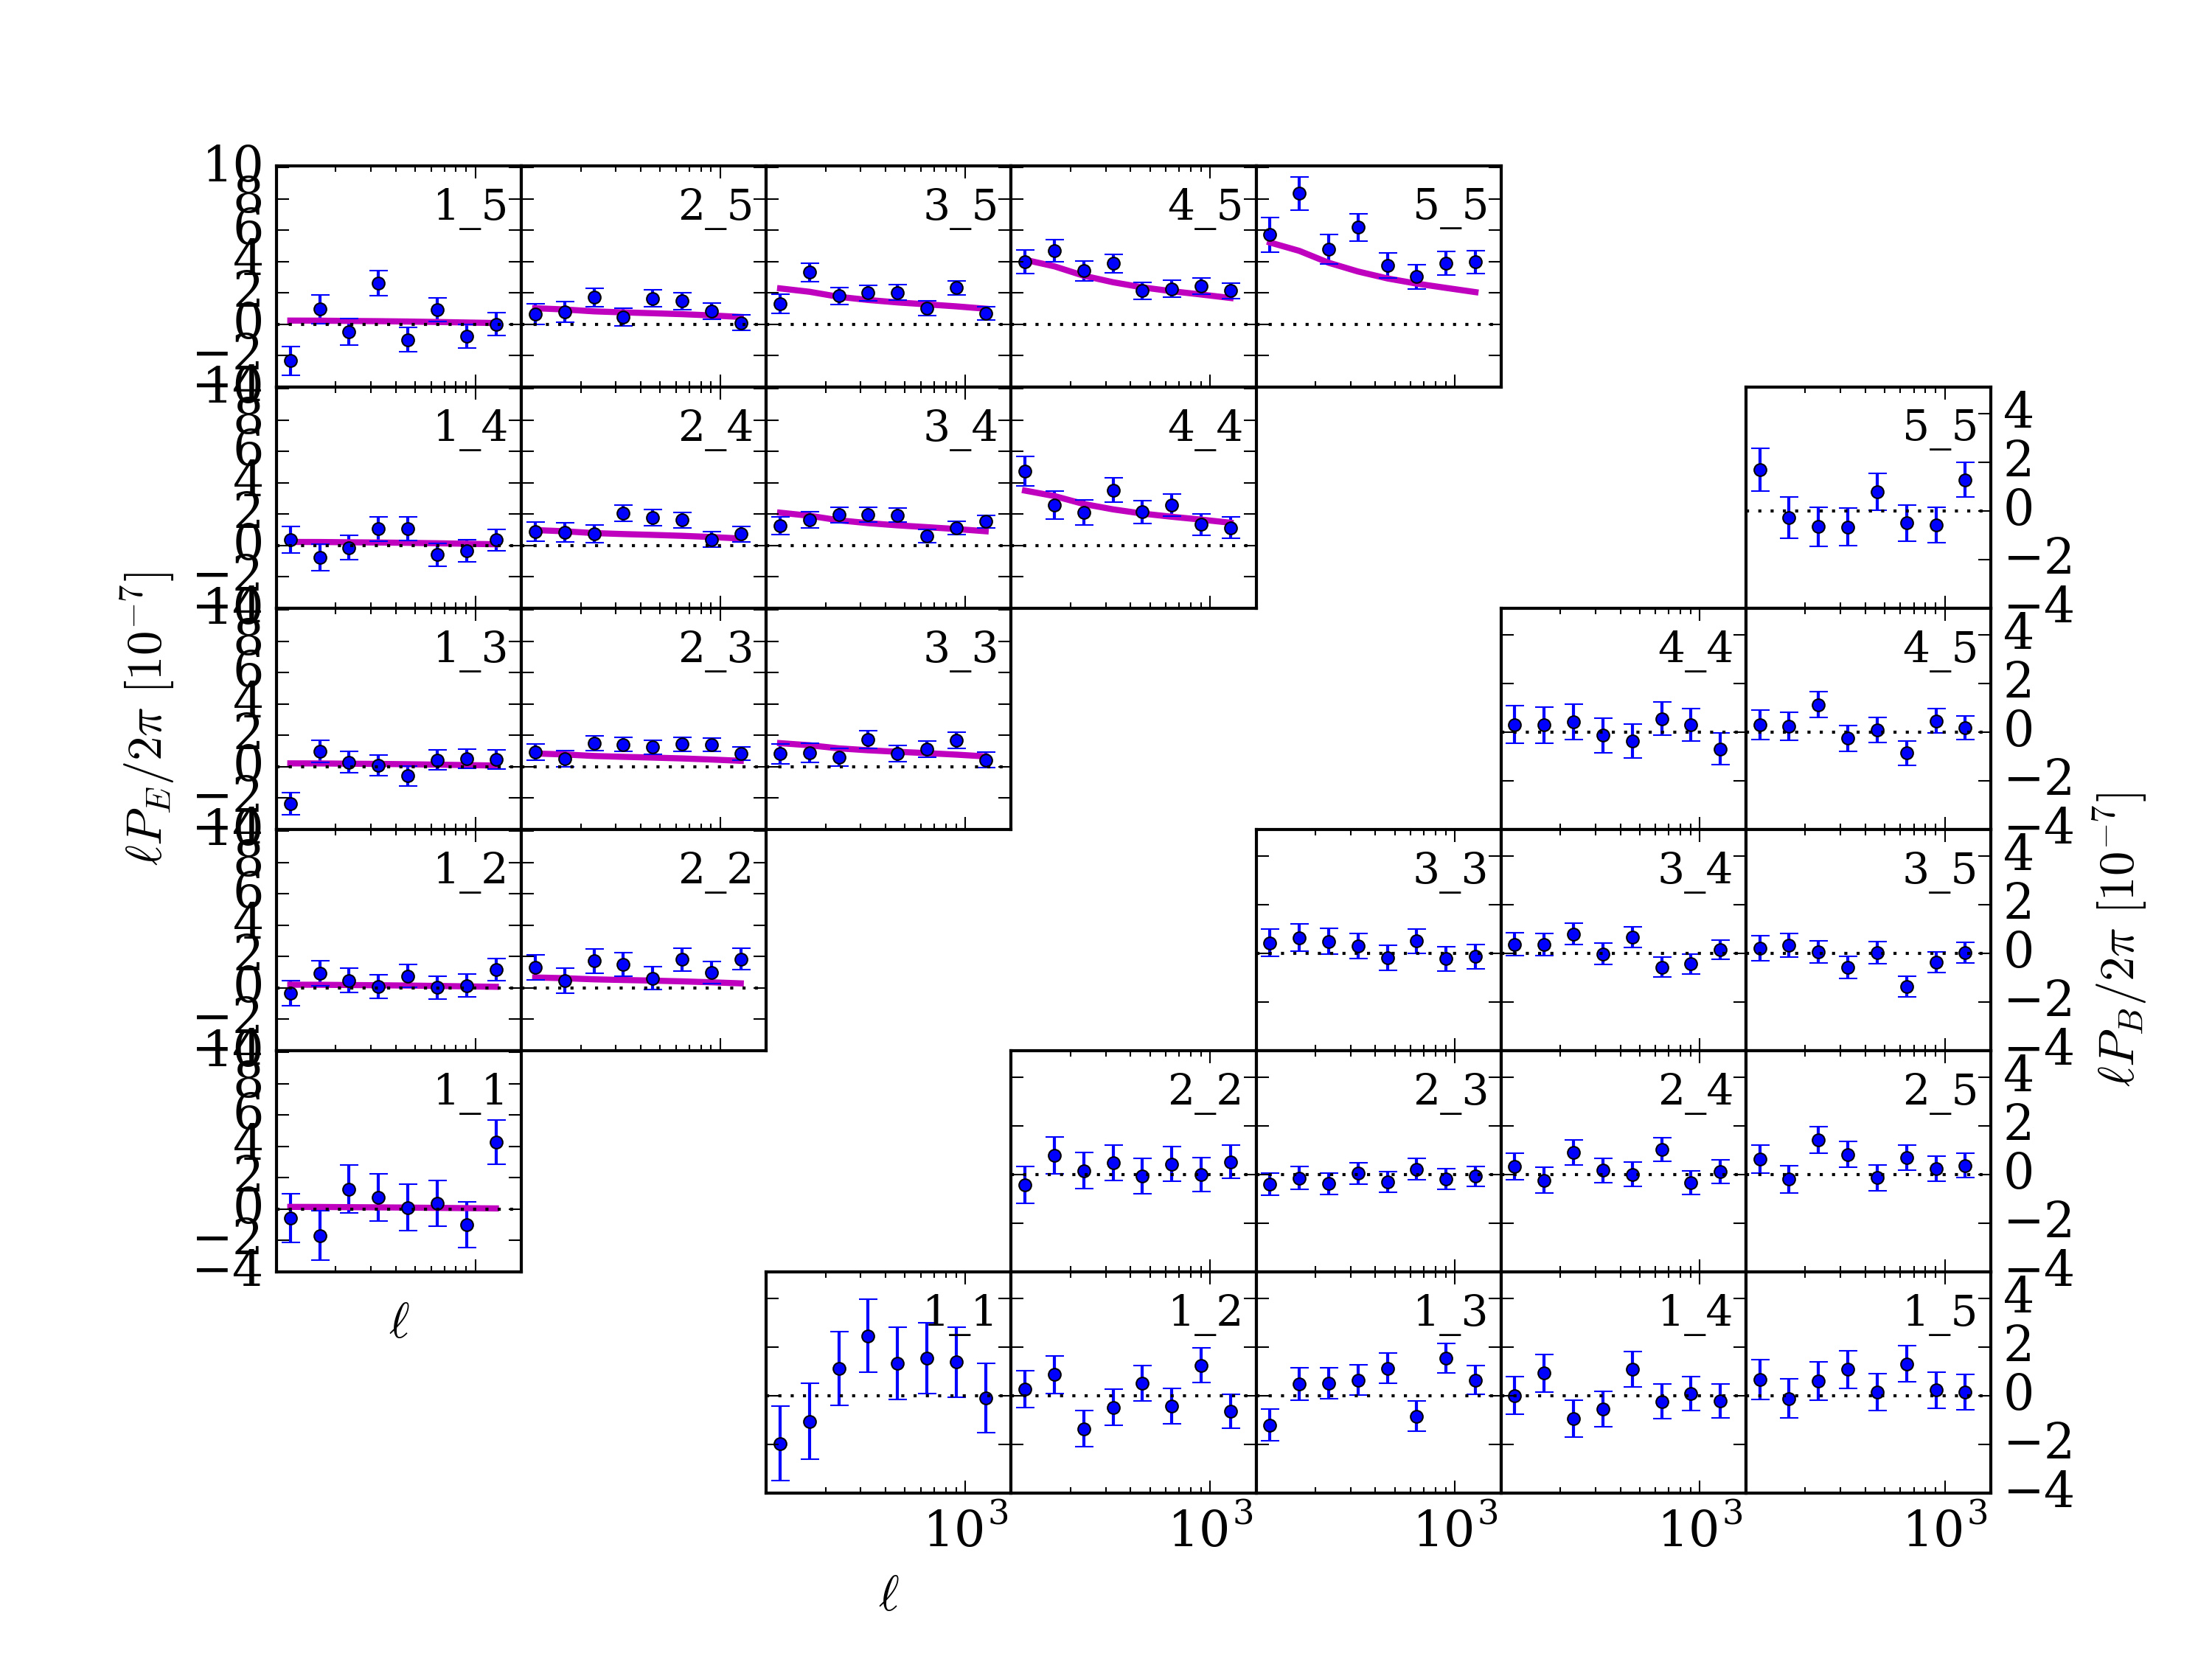
\includegraphics[width=\textwidth]{Data_Plots/Pkk/Pkk_K1000_2Dbins_v2_goldclasses_Flag_SOM_Fid.png}
        \caption{KiDS-1000 cosmic shear power spectra:  Tomographic
          band powers comparing the E-modes (upper left block) with the best-fit
          cosmological model from our combined multi-probe analysis
          \ch{TO DO}.  The tomographic
        bin combination is indicated in the upper right corner of each
      sub-panel.  The null-test B-modes (lower right block), are
      consistent with zero for both the full data vector, and each
     bin combination individually.}
        \label{fig:Pkk}
\end{figure*}

\subsection{Galaxy-Galaxy Lensing}
\label{sec:GGL}
Summary of Blake et al?


In Figure~\ref{fig:Pgk} we present the KiDS-1000 galaxy-galaxy lensing
power spectra, around lenses from the BOSS and 2dFLenS surveys.

\begin{figure*}
        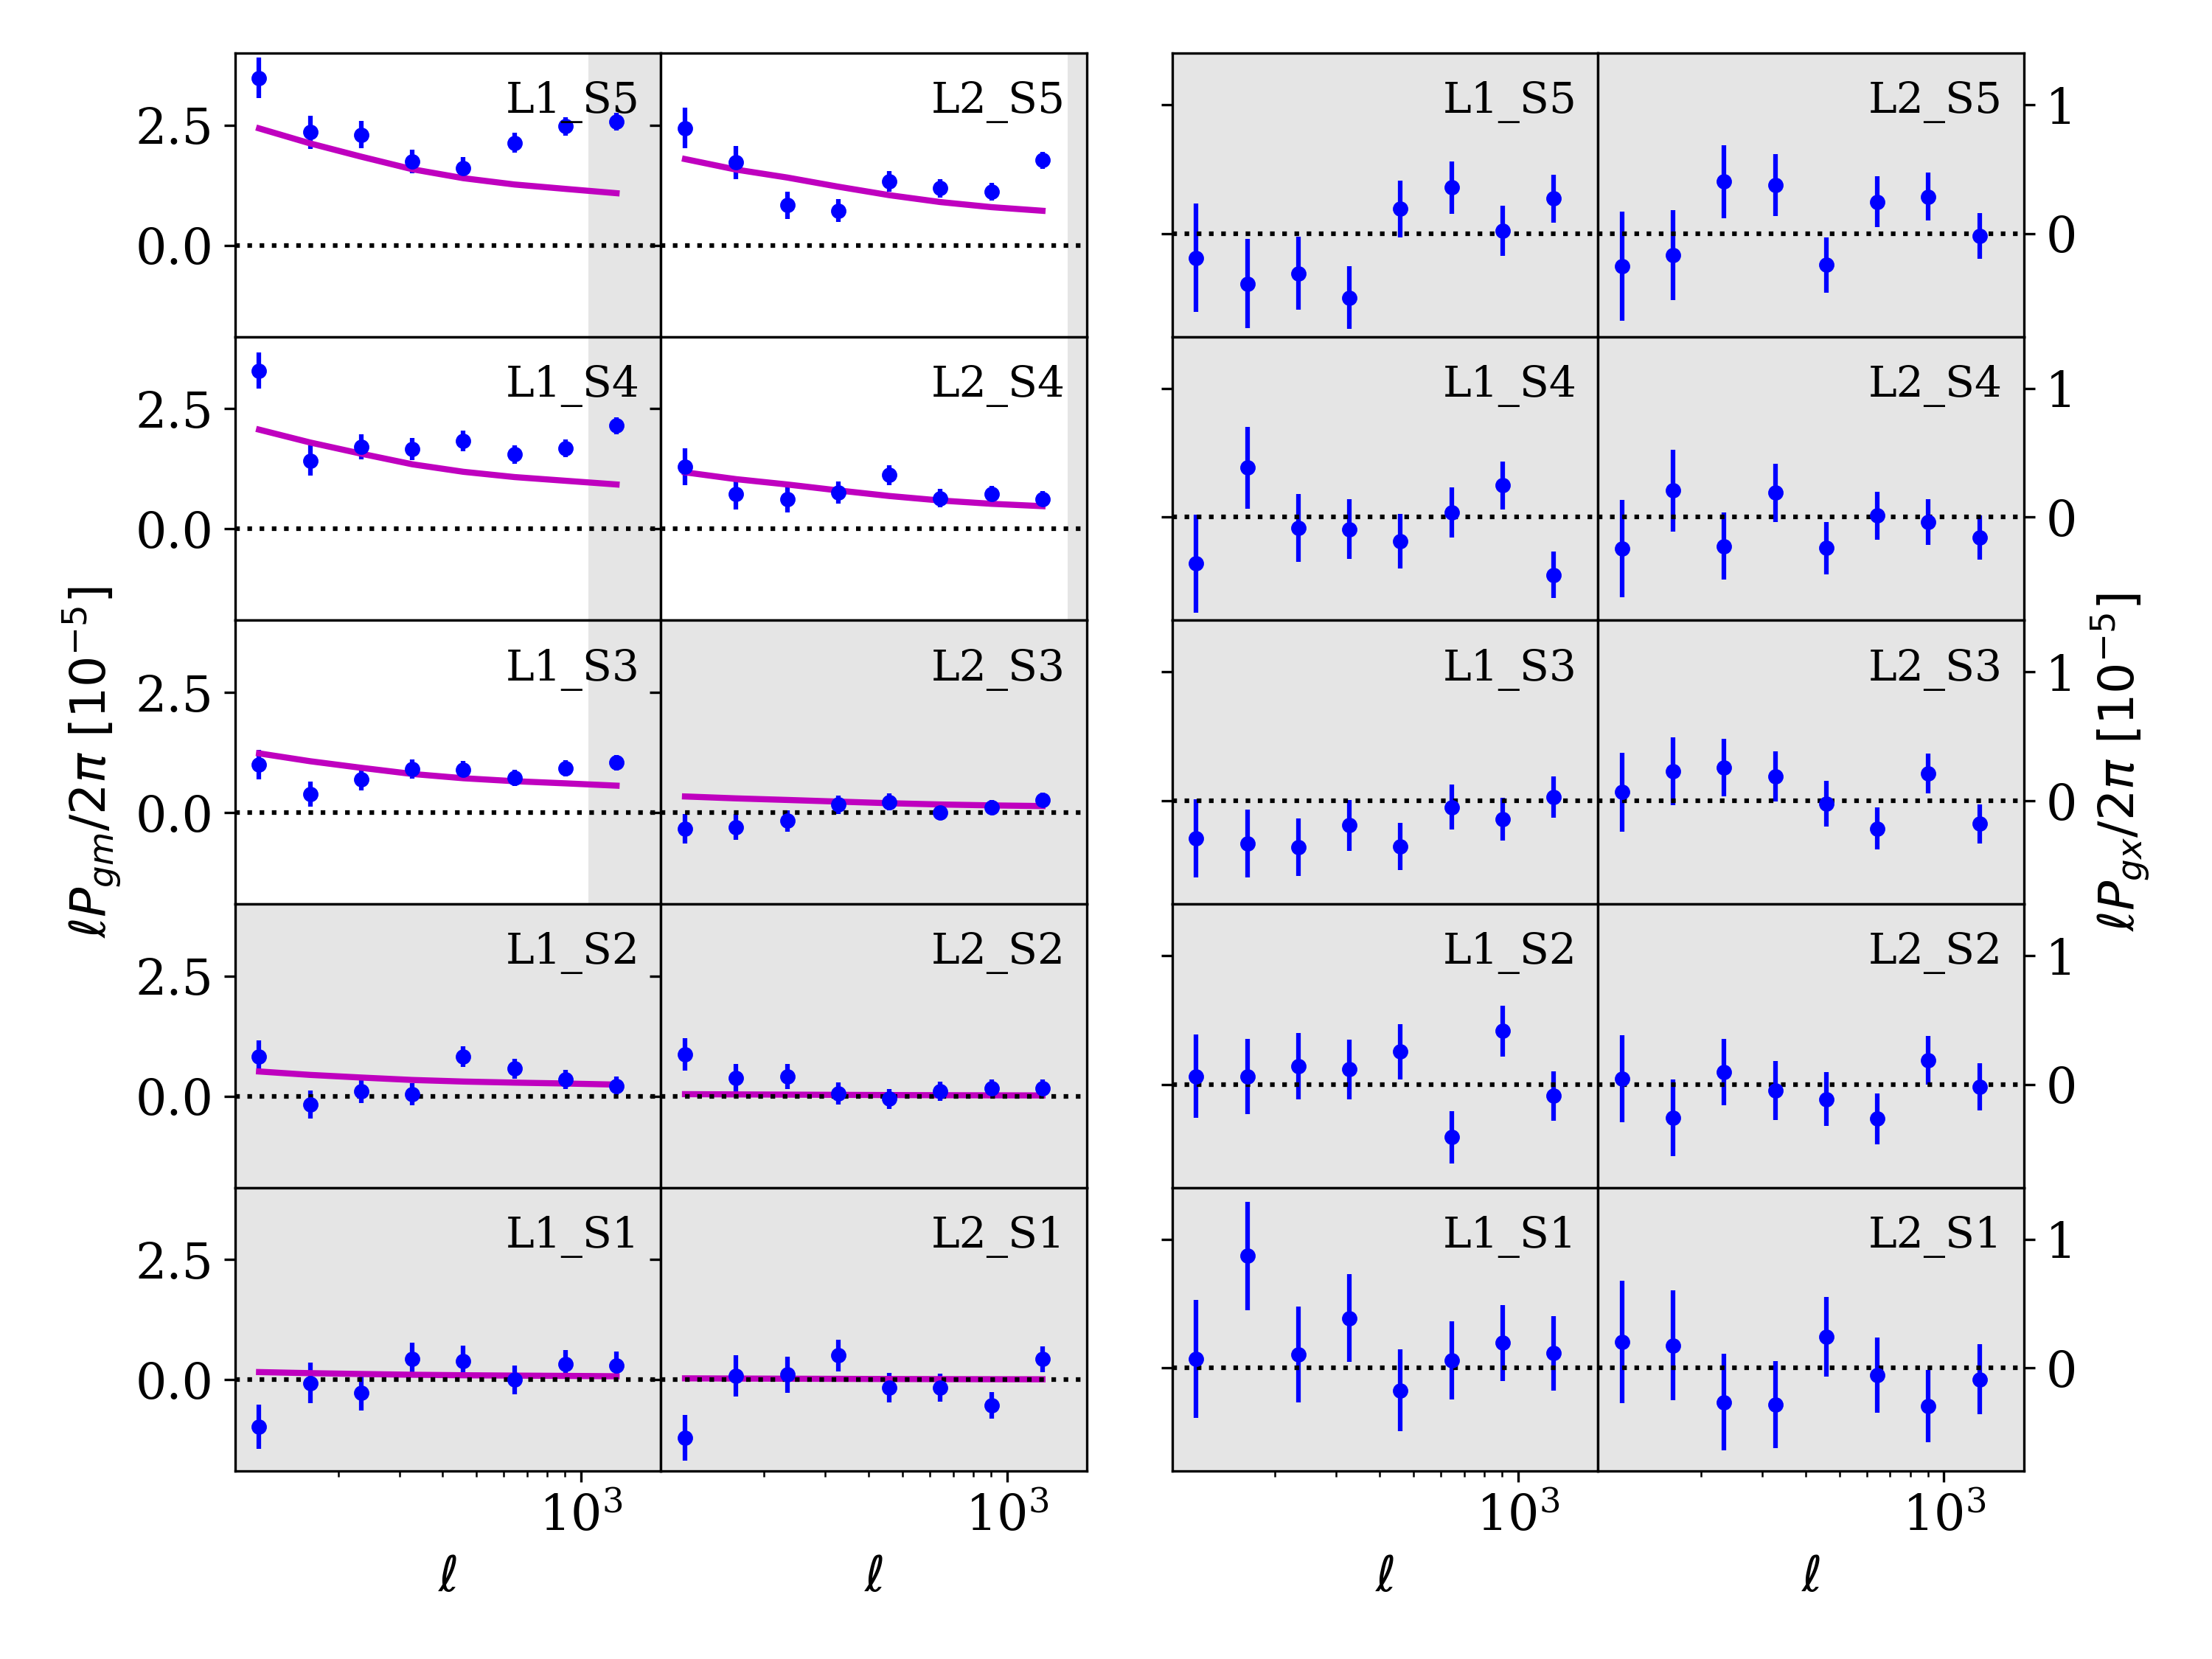
\includegraphics[width=\textwidth]{Data_Plots/Pgk/Pgk_K1000_2Dbins_v2_goldclasses_Flag_SOM_Fid.png}
        \caption{KiDS-1000 galaxy-galaxy lensing power spectra:
          Tomographic band powers comparing the E-modes (left block)
          with the best-fit
          cosmological model from our combined multi-probe analysis
          \ch{TO DO}.  The tomographic 
        bin combination of BOSS and 2dFLenS lenses (L) with KiDS-1000
        sources (S), is indicated in the upper right corner of each
        sub-panel.  Data within grey-regions are not included in the cosmological analysis.
        The null-test B-modes (right block), are
      consistent with zero for both the full data vector, and each
     bin combination individually \ch{TO DO}.}
        \label{fig:Pgk}
\end{figure*}

\subsection{Anisotropic Galaxy Clustering}
\label{sec:clustering}
Summary of \citet{sanchez/etal:2017}

In Figure~\ref{fig:wedges} we present the BOSS-DR12 anisotropic
clustering wedges.
\begin{figure*}
        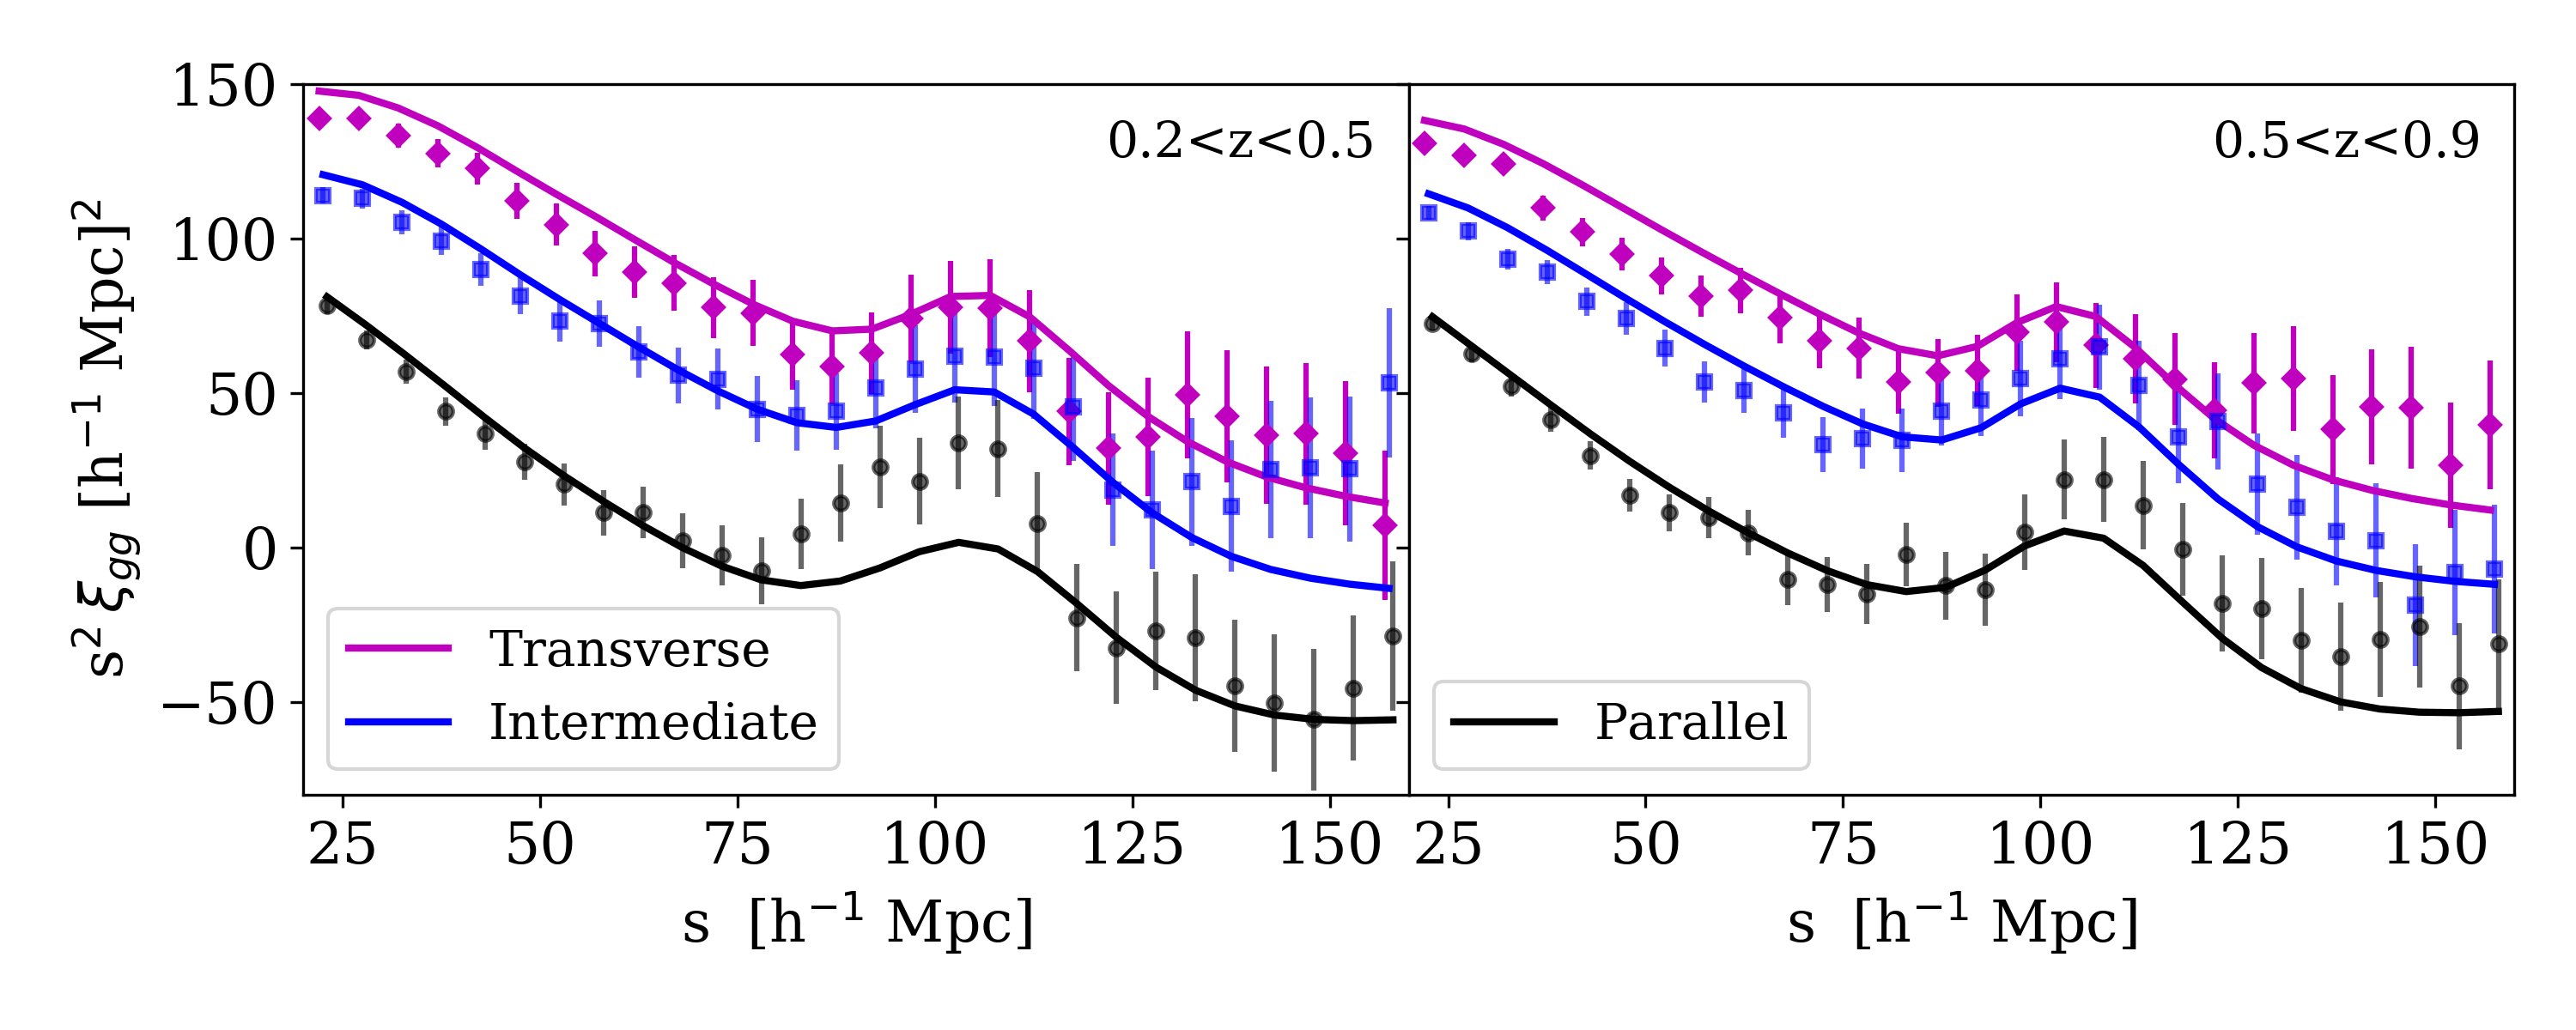
\includegraphics[width=\textwidth]{Data_Plots/clustering_wedges/BOSS_Sanchez_wedges.png}
        \caption{BOSS-DR12 anisotropic clustering from \citet{sanchez/etal:2017}:
          The transverse (pink), intermediate (blue) and parrallel
          (black) clustering wedges in two redshift bins, compared 
          with the best-fit
          cosmological model from our combined multi-probe analysis
          \ch{TO DO}.}
        \label{fig:wedges}
\end{figure*}

\subsection{Covariance}
\label{sec:Cov}
Summary of \citet{joachimi/etal:inprep}

